\section{Frequency Filtration}
\label{sec:filtering}
The previous section provides motivation for finding ways to reduce the
number of points in the signal and also the number of oscillators that the
signal contains. This has led to work on a procedure for generated
frequency-filtered ``sub-FIDs'' from the original data. A detailed description
of the filtering procedure is presented in this section.

\subsection{The \acl{VE}}
In brief, the filtering procedure  consists taking the \ac{FT} of the \ac{FID},
applying a band-pass filter on the spectral data to discard parts of not being
considered, and returning the spectrum back to the time-domain by an \ac{IFT}.
For a filtered \ac{FID} to be faithfully described by the model of a
summation of damped complex sinusoids, it is necessary that the
spectral peaks of interest lie effectively entirely within the filter
region\footnote{
    Lorentzian lineshapes tend to, but don't reach zero, as the distance from
    the maximum tends to $\infty$\cite{Tang1994}. However, as long as a
    sufficiently wide filtering is employed, the regions of the Lorentzian
    which do not pass through the filter can be assumed to be negligible.
}.
For absorptive Lorentzians, due to their characteristically narrow
linewidths, this is straightforward. However, for broader dispersive
Lorentzians, this is far more challenging. For this reason, generating
a spectrum in which only the real component is retained is desired.
Assuming the data has been phase-corrected, this will produce a
spectrum comprising only absorptive Lorentzians. The \ac{VE} has been employed
here, which has found application in the field of compressed sensing
NMR\cite{Mayzel2014,Golowicz2020,Luo2020}. This is a signal with double the
size as the original \ac{FID}, with the key characteristic that its \ac{FT} has
a real component which is equivalent to its counterpart derived from an
unaltered \ac{FID} (except it has double the points), and an imaginary
component of $0$s.

\subsubsection{The \acs{1D} \acl{VE}}
Assuming that a \ac{1D} \ac{FID} has been phase-corrected, such that $\bdphi =
\symbf{0} \in \mathbb{R}^M$, it can be denoted as
\begin{subequations}
    \begin{gather}
        \by =
        \symbf{\gamma} \odot
            \left(
                \symbf{c}^{(1)} + \iu \symbf{s}^{(1)}
            \right) + \bw, \\
        \symbf{\gamma} = \sum_m \bdam \exp \left(
                - \bdetaone \left[ m \right]
                \symbf{\tau}^{(1)}
            \right), \\
            \symbf{c}^{(1)}\text{/}\symbf{s}^{(1)} = \sum_m \cos\text{/}\sin \left(
                2 \pi \bdfone \left[ m \right] \symbf{\tau}^{(1)}_{\vphantom{t}}
            \right), \\
        \symbf{\tau}^{(1)} =
            \begin{bmatrix}
                0 & \Dtone & \cdots & \left(\None_{\vphantom{t}} - 1\right) \Dtone
            \end{bmatrix}\T
    \end{gather}
\end{subequations}
The frequency-dependence has been decomposed into its real and imaginary
components. With this in mind, a conjugate pair of signals are defined:
\begin{equation}
    \symbf{\psi}_{\pm} =
        \symbf{\gamma} \odot \left(
            \symbf{c}^{(1)} \pm \iu \symbf{s}^{(1)}
            \right) + \bw \equiv
            \Re\left(\by\right) \pm \iu \Im\left(\by\right)
\end{equation}
Two vectors $\lbrace \symbf{t}_{1}, \symbf{t}_2 \rbrace \in \mathbb{C}^{2
\None}$ are constructed using the conjugate pair:
\begin{itemize}
    \item $\symbf{t}_1$ is given by $\symbf{\psi}_+$ padded with zeros from below:
        \begin{equation}
            \symbf{t}_1 = \begin{bmatrix}
                \symbf{\psi}_+ \\ \symbf{0} \in \mathbb{C}^{\None}
            \end{bmatrix},\\
        \end{equation}
    \item $\symbf{t}_2$ is given by $\symbf{\psi}_{-}$ with its elements in
        reversed order ($\cdot^{{\leftrightsquigarrow}^{(1)}}$), padded with zeros
        from above, and finally subjected to a right circular shift by one
        element ($\cdot^{{\circlearrowright}^{(1)}}$):
        \begin{equation}
            \symbf{t}_2 = \begin{bmatrix}
                \symbf{0} \in \mathbb{C}^{\None} \\ \symbf{\psi}_-^{{\leftrightsquigarrow}^{(1)}}
        \end{bmatrix}^{{\circlearrowright}^{(1)}},
       \end{equation}
\end{itemize}
The \ac{VE} $\by_{\text{ve}}$ is then given by $\symbf{t}_1 +
\symbf{t}_2$, with the first element divided by $2$, which is equivalent to
\begin{equation}
    \by_{\text{ve}} =
    \begin{bmatrix}
        \Re\left( \by[0^{\vphantom{(1)}}] \right) &
        \by[1^{\vphantom{(1)}}] &
        \cdots &
        \by\left[\None - 1\right] &
        0 &
        \by\left[\None - 1\right]^* &
        \cdots &
        \by\left[1^{\vphantom{(1)}}\right]^*
    \end{bmatrix}\T.
\end{equation}
A signal of this form is illustrated in panel a of Figure \ref{fig:filtering}. As
eluded to already, the \ac{FT} of $\by_{\text{ve}}$ produces a spectrum
$\symbf{s}_{\text{ve}}$ such that $\Im\left(\symbf{s}_{\text{ve}}\right) =
\symbf{0}$, with $\Re\left(\symbf{s}_{\text{ve}}\right)$ featuring absorption
Lorentzian peaks (panel b of Figure \ref{fig:filtering}).

\begin{figure}
     \centering
     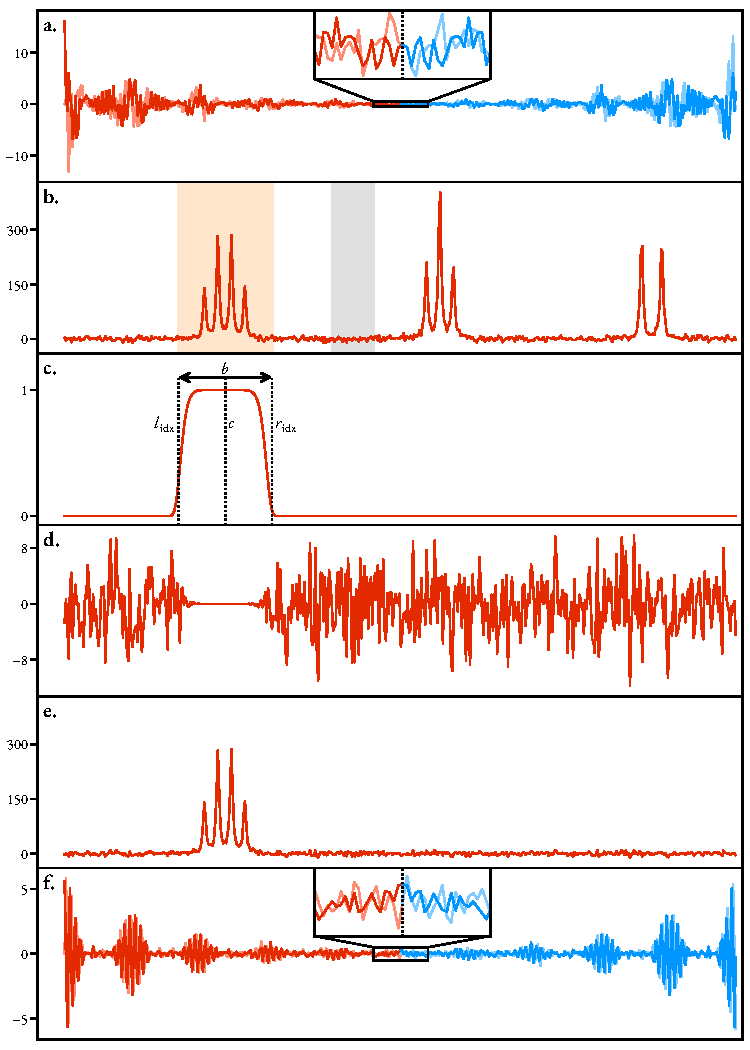
\includegraphics{filtering/filtering.pdf}
     \caption{
         An illustration of the filtering procedure applied to a \ac{1D}
         \ac{FID}.
         \textbf{a.} A \ac{VE} $\by_{\text{ve}}$, with the first and last
         $\None$ points coloured red and blue, respectively. The middle of the
         \ac{VE} is magnified to highlight its conjugate symmetry.
         \textbf{b.} The \ac{FT} of the \ac{VE}, $\symbf{s}_{\text{ve}}$.
         The region of interest (orange) and noise region (grey) are denoted.
         \textbf{c.} A super-Gaussian function used as a band-pass filter,
         $\symbf{g}$.
         \textbf{d.} \ac{AWGN} vector to be added to the filtered spectrum.
         The magnitude of the signal at each point is dependent on the
         corresponding super-Gaussian value.
         \textbf{e.} The filtered spectrum $\widetilde{\symbf{s}}_{\text{ve}}$,
         formed by applying the super-Gaussian filter, and adding the noise
         vector.
         \textbf{f.} The \ac{IFT} of the filtered spectrum,
         $\widetilde{\symbf{y}}_{\text{ve}}$, from which the final filtered
         signal $\widetilde{\symbf{y}}$ is obtained by extracting
         the first $\None$ points.
     }
     \label{fig:filtering}
 \end{figure}

\subsubsection{The \acs{2D} \acl{VE}}
The \ac{VE} concept can be generalised to any number of dimensions, assuming
that a pair of amplitude-modulated signals exist for each indirect-dimension,
thus requiring a set of $2^{D-1}$ signals for a $D$-dimensional dataset.
\note{Maybe describe the general case in the appendix if you're bold enough?}
For the
\ac{2D} case, this corresponds to the pair of signals $\lbrace \bY_{\cos},
\bY_{\sin} \rbrace$, given by \eqref{eq:general fid} with $D=2$ and $\zeta = \lbrace
\cos(\cdot), \sin(\cdot) \rbrace$, taking the forms (with noise neglected)
\begin{subequations}
    \begin{gather}
        \bY_{\cos} =
            \symbf{\Gamma} \odot
            \symbf{C}^{(1)} \odot \left(
                \symbf{C}^{(2)} +
                \iu \symbf{S}^{(2)}
            \right), \\
        \bY_{\sin} =
            \symbf{\Gamma} \odot
            \symbf{S}^{(1)} \odot \left(
                \symbf{C}^{(2)} +
                \iu \symbf{S}^{(2)}
            \right), \\
        \symbf{\Gamma} =
            \sum_m \bdam \left(
                \exp \left( -\bdetaonem \symbf{\tau}^{(1)} \right) \otimes
                \exp \left( -\bdetatwom \symbf{\tau}^{(2)} \right)
            \right), \\
        \symbf{C}^{(1)} \text{/} \symbf{S}^{(1)}
        = \sum_{m} \cos \text{/} \sin \left(2 \pi \bdfonem \symbf{\tau}^{(1)} \right)
            \otimes \symbf{1} \in \mathbb{C}^{\Ntwo}, \\
        \symbf{C}^{(2)} \text{/} \symbf{S}^{(2)} =
            \symbf{1} \in \mathbb{C}^{\None} \otimes
            \sum_{m} \cos \text{/} \sin \left(2 \pi \bdftwom \symbf{\tau}^{(2)} \right).
    \end{gather}
\end{subequations}
Four matrices are then constructed of the form
\begin{equation}
    \begin{gathered}
        \symbf{\Psi}_{\pm\pm} =
            \symbf{\Gamma} \odot \left(
                \symbf{C}^{(1)} \pm^{(1)} \hspace*{2pt} \iu \symbf{S}^{(1)}
                \right) \odot \left(
                    \symbf{C}^{(2)} \pm^{(2)} \hspace*{2pt} \iu \symbf{S}^{(2)}
                \right) \\
         \equiv
             \Re\left( \symbf{Y}_{\cos} \right)
             \pm^{(1)} \pm^{(2)} -
             \Im\left( \symbf{Y}_{\sin} \right)
             + \iu \left(
             \pm^{(1)}
             \Re\left( \symbf{Y}_{\sin} \right)
             \pm^{(2)}
             \Im\left( \symbf{Y}_{\cos} \right)
             \right),
    \end{gathered}
\end{equation}
from which the matrices $\symbf{T}_{1 \rightarrow 4} \in \mathbb{C}^{2 \None
\times 2 \Ntwo}$ are generated:
\begin{subequations}
    \begin{gather}
        \symbf{T}_1 =
        \begin{bmatrix}
            \symbf{\Psi}_{++} & \symbf{0} \\
            \symbf{0} & \symbf{0}
        \end{bmatrix}, \\
        \symbf{T}_2 =
        \begin{bmatrix}
            \symbf{0} & \symbf{0} \\
            \symbf{\Psi}_{-+}^{\leftrightsquigarrow (1)} & \symbf{0}
        \end{bmatrix}^{\circlearrowright (1)}, \\
        \symbf{T}_3 =
        \begin{bmatrix}
            \symbf{0} & \symbf{\Psi}_{+-}^{\leftrightsquigarrow (2)} \\
            \symbf{0} & \symbf{0}
        \end{bmatrix}^{\circlearrowright (2)}, \\
        \symbf{T}_4 =
        \begin{bmatrix}
            \symbf{0} & \symbf{0} \\
            \symbf{0} & \symbf{\Psi}_{--}^{\leftrightsquigarrow (1,2)}
        \end{bmatrix}^{\circlearrowright (1,2)}.
    \end{gather}
\end{subequations}
\note{Appendix for explicit forms of the matrices $\symbf{T}_{1-4}$}
The virtual echo is then given by $\symbf{Y}_{\text{ve}} = \sum_{i=1}^4
\symbf{T}_i$, with the first row and column divided by two. For a full outline
of the 2D filtering procedure, see Algorithm \ref{alg:filter-2d}.

\subsection{The filtering process}
Having constructed a virtual echo $\symbf{Y}_{\text{ve}} \in \mathbb{C}^{2\None
\times \cdots \times 2\ND}$, a spectrum with absorption Lorentzians is produced
with $\symbf{S}_{\text{ve}} = \FT\left(\symbf{Y}_{\text{ve}}\right)$. To filter
the spectrum, it is subjected to element-wise multiplication with a
super-Gaussian function. The super-Gaussian is defined by a centre
$c^{(d)} \in \mathbb{R}: 0 < c^{(d)} < 2 \Nd$ and a bandwidth  $b^{(d)} \in
\mathbb{N}: b^{(d)} < 2\Nd$ in each dimension (panel c of Figure
\ref{fig:filtering}):
\begin{subequations}
    \begin{gather}
        \symbf{G} = \bigotimes_{d=1}^D
            \symbf{g}^{(d)}, \\
        \symbf{g}_{\vphantom{t}}^{(d)}\left[ \nd \right] = \exp \left(
            -2^{p+1} \left(
                \frac{\nd - c^{(d)}_{\vphantom{t}}}{b^{(d)}}
            \right)^p
        \right)\ \forall \nd \in \lbrace 0, \cdots, 2 \Nd - 1 \rbrace.
        \label{eq:super-Gaussian-onedim}
    \end{gather}
\end{subequations}
An example of a \ac{1D} super-Gaussian is given in panel $c$ of Figure
\ref{fig:filtering}. The scalar $p \in \mathbb{R}_{>0}$ dictates the steepness
of the filter at the boundaries, with the function becoming more ``box-like''
as it increases. It is set to $40$ in this work and as the default in
\ac{EsPy}. Application of the super-Gaussian filter to $\symbf{S}_{\text{ve}}$
would lead to large sections of the filtered spectrum being $0$. This has an
undesired impact on the \ac{MDL}, as noise that has passed through filter (i.e.
the noise inside the region of interest) will now seem to resemble true signal,
as its amplitude is infinitely greater than the zeroed regions. A massive
over-estimation of model order therefore result. In order to obtain better
results from the model order selection, an array of synthetic \ac{AWGN} is
added to the filtered spectrum. To achieve this, a region in
$\symbf{S}_{\text{ve}}$ is specified which contains no discernible signal peaks
(referred to as the \emph{noise region}). The variance of this region
$\sigma^2$ is determined, and used to construct an array of values sampled from
a normal distribution with mean $0$ and variance $\sigma^2$,
$\symbf{W}_{\sigma^2} \in \mathbb{R}^{2 \None \times \cdots \times 2 \ND}$.
The filtered spectrum is then given by
\begin{equation}
    \widetilde{\symbf{S}}_{\text{ve}} = \symbf{S}_{\text{ve}} \odot \symbf{G} + \symbf{W}_{\sigma^2} \odot \left(\symbf{1} - \symbf{G} \right).
    \label{eq:Sve-tilde}
\end{equation}
Note that the noise array's magnitude at each point is attenuated by the value
of the super-Gaussian filter. Inside the region of interest ($\symbf{G}\left[
\none, \cdots, \nD \right] = 1$ ), the noise is nullified. See panel d of
Figure \ref{fig:filtering} for an example.

After filtering, $\widetilde{\symbf{S}}_{\text{ve}}$ is returned to the
time-domain by \ac{IFT}. The \ac{IFT} of a real-valued spectrum generates a
conjugate-symmetric signal. This is sliced in half in each dimension,
generating the final filtered sub-FID $\widetilde{\bY} \in
\mathbb{C}^{\None \times \cdots \times \ND}$:
\begin{equation}
    \widetilde{\bY} =
        \frac{1}{2^{D-1}}
        \IFT\left(\widetilde{\symbf{S}}_{\text{ve}}\right)
        \left[0:\None, \cdots, 0:\ND\right].
        \label{eq:yve-tilde}
\end{equation}
The scaling factor in \eqref{eq:yve-tilde} is to account for how many signals
have been combined to generate the \ac{VE}.

\subsubsection{Determining $c^{(d)}$ and  $b^{(d)}$}
The central index and bandwidth of the super-Gaussian filter function are given by the following expressions:
\begin{subequations}
    \begin{gather}
        c_{\vphantom{\text{idx}}}^{(d)} = \tfrac{1}{2} \left(l^{(d)}_{\text{idx}} + r^{(d)}_{\text{idx}}\right), \\
        b_{\vphantom{\text{idx}}}^{(d)} = l^{(d)}_{\text{idx}} - r^{(d)}_{\text{idx}},
    \end{gather}
\end{subequations}
where $l^{(d)}_{\text{idx}}$ and $r^{(d)}_{\text{idx}}$ denote the desired
indices where the filter's left and right bounds are located, respectively.
Array indices can be obtained from the corresponding spectral frequency
$f^{(d)}_{\unit{\hertz}}$ via
\begin{equation}
    \begin{gathered}
        f_{\text{idx}}^{(d)} =
            \left \lfloor
                \frac
                {
                    \left(2 \Nd_{\vphantom{d}} - 1\right)
                    \left(\fswd + 2 \left(\foffd - f_{\unit{\hertz}}^{(d)}\right) \right)
                }
                {2 \fswd}
            \right \rceil \\
        \forall f^{(d)}_{\unit{\hertz}} \in
            \left[\foffd - \tfrac{1}{2} \fswd, \foffd + \tfrac{1}{2} \fswd\right].
        \label{eq:fidx}
    \end{gathered}
\end{equation}
Conversion from \unit{\partspermillion} to array indices can be achieved by
replacing  $f_{\unit{\hertz}}$ in \eqref{eq:fidx} with
$f_{\unit{\partspermillion}} f_{\text{sfo}}$, where $f_{\text{sfo}}$ is the
transmitter frequency (\unit{\mega \hertz}).

\subsubsection{Spectrum slicing}
Thus far, the method described is able to reduce the model order of a given
signal, however the signal still comprises the same number of points. However
it is clear that there are a large number of points outside the region of
interest in $\widetilde{\symbf{S}}_{\text{ve}}$ that do not possess any
meaningful information. Discarding such points should then lead to filtered
\ac{FID} with the same information about the resonances of interest, but with
far fewer points. A slicing ratio is defined, $\xi \in \mathbb{R}: \xi > 1$,
which dictates the left and right indices at which the spectrum should be sliced
in each dimension:
\begin{subequations}
    \begin{gather}
        l_{\text{slice}}^{(d)} =
        \begin{cases}
            c_{\text{idx}}^{(d)} - \left \lfloor \frac{b^{(d)} \xi}{2} \right \rfloor &
            \text{if } \geq 0 \\
            0 & \text{otherwise}
        \end{cases} \\
        r_{\text{slice}}^{(d)} =
        \begin{cases}
            c_{\text{idx}}^{(d)} + \left \lceil \frac{b^{(d)} \xi}{2} \right \rceil &
            \text{if } \leq 2 \Nd - 1 \\
            2 \Nd - 1 & \text{otherwise}
        \end{cases}
    \end{gather}
\end{subequations}
The filtered spectrum is then sliced accordingly:
\begin{equation}
    \widetilde{\symbf{S}}_{\text{ve, slice}} =
        \widetilde{\symbf{S}}_{\text{ve}} \left[
            l_{\text{slice}}^{(1)} :
            r_{\text{slice}}^{(1)} + 1,
            \cdots,
            l_{\text{slice}}^{(D)} :
            r_{\text{slice}}^{(D)} + 1
        \right].
\end{equation}
The equivalent process is applied to $\widetilde{\symbf{S}}_{\text{ve,slice}}$
to generate the final filtered sub-\ac{FID}: \ac{IFT} followed by slicing in
half in each dimension.  It is also necessary to scale the signal by the ratio
of the number of points in the sliced spectrum and it's unsliced counterpart.
\begin{subequations}
    \begin{gather}
        \widetilde{\bY} =
            \prod_{d=1}^D \left(\frac{r_{\text{slice}}^{(d)} - l_{\text{slice}}^{(d)}}{2 \Nd}\right)
            \IFT \left( \widetilde{\symbf{S}}_{\text{ve, slice}} \right)
            \left[
                0 : \None_{\text{slice}}, \cdots, 0 : \ND_{\text{slice}}
            \right] \\
            \Nd_{\text{slice}} = \left \lfloor \frac{r_{\text{slice}}^{(d)} - l_{\text{slice}}^{(d)}}{2} \right \rfloor
    \end{gather}
\end{subequations}
Finally, the effective sweep widths and transmitter offsets will have been
altered by this process. The corrected values can be computed using
\begin{subequations}
    \begin{gather}
        f_{\text{sw,slice}}^{(d)} = \frac{r_{\text{slice}}^{(d)} - l_{\text{slice}}^{(d)}}{2 \Nd - 1} \fswd \\
        f_{\text{off,slice}}^{(d)} = \foffd + \frac{\fswd}{2} \left( 1 - \frac{l_{\text{slice}}^{(d)} + r_{\text{slice}}^{(d)}}{2 \Nd - 1}\right)
    \end{gather}
\end{subequations}
